\RequirePackage{atbegshi}
\documentclass[compress,aspectratio=169]{beamer}\usepackage[]{graphicx}\usepackage[]{color}
% maxwidth is the original width if it is less than linewidth
% otherwise use linewidth (to make sure the graphics do not exceed the margin)
\makeatletter
\def\maxwidth{ %
  \ifdim\Gin@nat@width>\linewidth
    \linewidth
  \else
    \Gin@nat@width
  \fi
}
\makeatother

\definecolor{fgcolor}{rgb}{0.345, 0.345, 0.345}
\makeatletter
\@ifundefined{AddToHook}{}{\AddToHook{package/xcolor/after}{\definecolor{fgcolor}{rgb}{0.345, 0.345, 0.345}}}
\makeatother
\newcommand{\hlnum}[1]{\textcolor[rgb]{0.686,0.059,0.569}{#1}}%
\newcommand{\hlstr}[1]{\textcolor[rgb]{0.192,0.494,0.8}{#1}}%
\newcommand{\hlcom}[1]{\textcolor[rgb]{0.678,0.584,0.686}{\textit{#1}}}%
\newcommand{\hlopt}[1]{\textcolor[rgb]{0,0,0}{#1}}%
\newcommand{\hlstd}[1]{\textcolor[rgb]{0.345,0.345,0.345}{#1}}%
\newcommand{\hlkwa}[1]{\textcolor[rgb]{0.161,0.373,0.58}{\textbf{#1}}}%
\newcommand{\hlkwb}[1]{\textcolor[rgb]{0.69,0.353,0.396}{#1}}%
\newcommand{\hlkwc}[1]{\textcolor[rgb]{0.333,0.667,0.333}{#1}}%
\newcommand{\hlkwd}[1]{\textcolor[rgb]{0.737,0.353,0.396}{\textbf{#1}}}%
\let\hlipl\hlkwb

\usepackage{framed}
\makeatletter
\newenvironment{kframe}{%
 \def\at@end@of@kframe{}%
 \ifinner\ifhmode%
  \def\at@end@of@kframe{\end{minipage}}%
  \begin{minipage}{\columnwidth}%
 \fi\fi%
 \def\FrameCommand##1{\hskip\@totalleftmargin \hskip-\fboxsep
 \colorbox{shadecolor}{##1}\hskip-\fboxsep
     % There is no \\@totalrightmargin, so:
     \hskip-\linewidth \hskip-\@totalleftmargin \hskip\columnwidth}%
 \MakeFramed {\advance\hsize-\width
   \@totalleftmargin\z@ \linewidth\hsize
   \@setminipage}}%
 {\par\unskip\endMakeFramed%
 \at@end@of@kframe}
\makeatother

\definecolor{shadecolor}{rgb}{.97, .97, .97}
\definecolor{messagecolor}{rgb}{0, 0, 0}
\definecolor{warningcolor}{rgb}{1, 0, 1}
\definecolor{errorcolor}{rgb}{1, 0, 0}
\makeatletter
\@ifundefined{AddToHook}{}{\AddToHook{package/xcolor/after}{
\definecolor{shadecolor}{rgb}{.97, .97, .97}
\definecolor{messagecolor}{rgb}{0, 0, 0}
\definecolor{warningcolor}{rgb}{1, 0, 1}
\definecolor{errorcolor}{rgb}{1, 0, 0}
}}
\makeatother
\newenvironment{knitrout}{}{} % an empty environment to be redefined in TeX

\usepackage{alltt} % aspectratio=169


% % % % % % % % % % % % % % %
%             MY PACKAGES 
% % % % % % % % % % % % % % %
\usepackage{graphicx}       % Use pdf, png, jpg, or eps with pdflatex; use eps in DVI mode
\usepackage{dcolumn} % this pack is neccesary to build nicer columns with texreg--dont remove it.
\usepackage[export]{adjustbox}
\usepackage{xcolor}[dvipsnames]
\usepackage{amssymb,amsmath}
\usepackage{threeparttable} % package to have long notes in reg tables in texreg. 

\usepackage{pgfplots}
\pgfplotsset{compat=1.11}
\usepgfplotslibrary{fillbetween}

%\usepackage{tipx}
%\usepackage{tikz}
%\usetikzlibrary{arrows,shapes,decorations.pathmorphing,backgrounds,positioning,fit,petri}
\usepackage{rotating}
%\usepackage{scalerel} % for inline images
\usepackage{import}
%\usepackage{times}
\usepackage{array}
\usepackage{tabularx}
%\usepackage{booktabs}
%\usepackage{textcomp}
\usepackage{float}
%\usepackage{setspace}      % \doublespacing \singlespacing \onehalfspacing %doble espacio
%\label{x:y}                          %ocupar para autoref.
%\autoref{x:y}                        %ocupar para autoref.
%\usepackage{nopageno}      %desactivar para p�ginas
\usepackage{pifont}
%\usepackage{marvosym} %faces
\usepackage{hyperref}
\usepackage{multirow}

\usepackage{tikz}
\usetikzlibrary{arrows,decorations.pathreplacing}



\usepackage{listings}
\usepackage{color}
\definecolor{dkgreen}{rgb}{0,0.6,0}
\definecolor{gray}{rgb}{0.5,0.5,0.5}
\definecolor{mauve}{rgb}{0.58,0,0.82}
\lstset{ %
  language=R,                     % the language of the code
  basicstyle=\TINY,           % the size of the fonts that are used for the code
  numbers=left,                   % where to put the line-numbers
  numberstyle=\tiny\color{gray},  % the style that is used for the line-numbers
  stepnumber=1,                   % the step between two line-numbers. If it's 1, each line
                                  % will be numbered
  numbersep=5pt,                  % how far the line-numbers are from the code
  backgroundcolor=\color{white},  % choose the background color. You must add \usepackage{color}
  showspaces=false,               % show spaces adding particular underscores
  showstringspaces=false,         % underline spaces within strings
  showtabs=false,                 % show tabs within strings adding particular underscores
  frame=single,                   % adds a frame around the code
  rulecolor=\color{black},        % if not set, the frame-color may be changed on line-breaks within not-black text (e.g. commens (green here))
  tabsize=1,                      % sets default tabsize to 2 spaces
  captionpos=b,                   % sets the caption-position to bottom
  breaklines=true,                % sets automatic line breaking
  breakatwhitespace=false,        % sets if automatic breaks should only happen at whitespace
  title=\lstname,                 % show the filename of files included with \lstinputlisting;
                                  % also try caption instead of title
  keywordstyle=\color{blue},      % keyword style
  commentstyle=\color{dkgreen},   % comment style
  stringstyle=\color{mauve},      % string literal style
  escapeinside={\%*}{*)},         % if you want to add a comment within your code
  morekeywords={*,...}            % if you want to add more keywords to the set
} 

% % % % % % % % % % % % % % %
%           PACKAGE CUSTOMIZATION
% % % % % % % % % % % % % % %

% GENERAL CUSTOMIZATION
\usepackage[math]{iwona}% font
\usetheme{Singapore}  % template I should use
%\usetheme{Szeged}  % alternative template
\usecolortheme{rose}  % color template
\makeatletter     % to show subsection/section title (1/3)
\beamer@theme@subsectiontrue % to show subsection/section title (2/3)
\makeatother      % to show subsection/section title (3/3)



% THIS BELOW IS TO MAKE NAVIGATION DOTS MARKED DURING PRESENTATION
\makeatletter
\def\slideentry#1#2#3#4#5#6{%
  %section number, subsection number, slide number, first/last frame, page number, part number
  \ifnum#6=\c@part\ifnum#2>0\ifnum#3>0%
    \ifbeamer@compress%
      \advance\beamer@xpos by1\relax%
    \else%
      \beamer@xpos=#3\relax%
      \beamer@ypos=#2\relax%
    \fi%
  \hbox to 0pt{%
    \beamer@tempdim=-\beamer@vboxoffset%
    \advance\beamer@tempdim by-\beamer@boxsize%
    \multiply\beamer@tempdim by\beamer@ypos%
    \advance\beamer@tempdim by -.05cm%
    \raise\beamer@tempdim\hbox{%
      \beamer@tempdim=\beamer@boxsize%
      \multiply\beamer@tempdim by\beamer@xpos%
      \advance\beamer@tempdim by -\beamer@boxsize%
      \advance\beamer@tempdim by 1pt%
      \kern\beamer@tempdim
      \global\beamer@section@min@dim\beamer@tempdim
      \hbox{\beamer@link(#4){%
          \usebeamerfont{mini frame}%
          \ifnum\c@section>#1%
            %\usebeamercolor[fg]{mini frame}%
            %\usebeamertemplate{mini frame}%
            \usebeamercolor{mini frame}%
            \usebeamertemplate{mini frame in other subsection}%
          \else%
            \ifnum\c@section=#1%
              \ifnum\c@subsection>#2%
                \usebeamercolor[fg]{mini frame}%
                \usebeamertemplate{mini frame}%
              \else%
                \ifnum\c@subsection=#2%
                  \usebeamercolor[fg]{mini frame}%
                  \ifnum\c@subsectionslide<#3%
                    \usebeamertemplate{mini frame in current subsection}%
                  \else%
                    \usebeamertemplate{mini frame}%
                  \fi%
                \else%
                  \usebeamercolor{mini frame}%
                  \usebeamertemplate{mini frame in other subsection}%
                \fi%
              \fi%
            \else%
              \usebeamercolor{mini frame}%
              \usebeamertemplate{mini frame in other subsection}%
            \fi%
          \fi%
        }}}\hskip-10cm plus 1fil%
  }\fi\fi%
  \else%
  \fakeslideentry{#1}{#2}{#3}{#4}{#5}{#6}%
  \fi\ignorespaces
  }
\makeatother


%%% bib begin
\usepackage[backend=biber,style=numeric, citestyle=ieee]{biblatex}
\addbibresource{/Users/hectorbahamonde/Bibliografia_PoliSci/library.bib} 


% USAGES
%% use \textcite to cite normal
%% \parencite to cite in parentheses
%% \footcite to cite in footnote
%% the default can be modified in autocite=FOO, footnote, for ex. 
%%% bib end



% % % % % % % % % % % % % % %
%       To show the TITLE at the Bottom of each slide
% % % % % % % % % % % % % % %

\beamertemplatenavigationsymbolsempty 
\makeatletter
\setbeamertemplate{footline}
{
\leavevmode%
\hbox{%
\begin{beamercolorbox}[wd=1\paperwidth,ht=2.25ex,dp=2ex,center]{title in head/foot}%
\usebeamerfont{title in head/foot}\insertshorttitle
\end{beamercolorbox}%
\begin{beamercolorbox}[wd=1
\paperwidth,ht=2.25ex,dp=2ex,center]{date in head/foot}%
\end{beamercolorbox}}%
}
\makeatother



% to switch off navigation bullets
%% using \miniframeson or \miniframesoff
\makeatletter
\let\beamer@writeslidentry@miniframeson=\beamer@writeslidentry
\def\beamer@writeslidentry@miniframesoff{%
  \expandafter\beamer@ifempty\expandafter{\beamer@framestartpage}{}% does not happen normally
  {%else
    % removed \addtocontents commands
    \clearpage\beamer@notesactions%
  }
}
\newcommand*{\miniframeson}{\let\beamer@writeslidentry=\beamer@writeslidentry@miniframeson}
\newcommand*{\miniframesoff}{\let\beamer@writeslidentry=\beamer@writeslidentry@miniframesoff}
\makeatother

% Image full size: use 
%%\begin{frame}
  %%\fullsizegraphic{monogram.jpg}
%%\end{frame}
\newcommand<>{\fullsizegraphic}[1]{
  \begin{textblock*}{0cm}(-1cm,-3.78cm)
  \includegraphics[width=\paperwidth]{#1}
  \end{textblock*}
}


% hyperlinks
\hypersetup{colorlinks,
            urlcolor=[rgb]{0.01, 0.28, 1.0},
            linkcolor=[rgb]{0.01, 0.28, 1.0}}



%\newcommand{\vitem}[]{\vfill \item}

% % % % % % % % % % % % % % %
%           DOCUMENT ID
% % % % % % % % % % % % % % %

\title{\input{title.txt}\unskip} % 


\author[shortname]{Hector Bahamonde \inst{1} \and Outi Sarpila \inst{1}}

\institute[shortinst]{\inst{1} University of Turku, Finland}

\date{April 7th, 2022}

%to to see shadows of previous blocks
%\setbeamercovered{dynamic}
\IfFileExists{upquote.sty}{\usepackage{upquote}}{}
\begin{document}














% % % % % % % % % % % % % % %
%           CONTENT
% % % % % % % % % % % % % % %

%% title frame
\begin{frame}
\titlepage
\end{frame}


\section{Introduction}
\subsection{Order of the day}

\begin{frame}[c]{}
  \begin{itemize}
    \item {\bf Motivate the problem}: It's clear that {\bf the better the candidate's looks, the higher the turnout}.

    \item {\bf Gaps in the literature}: The literature \emph{only} looks at candidate attractiveness, which is just \emph{one} dimension of physical appearance.

\item Our paper:

      \begin{itemize}
        \item {\bf Beyond attractiveness}: explore the degree in which {\bf a candidate's occupation is congruent with his/her physical appearance}.
        \item {\bf Inequality perspective}: Study how the candidate's perceived {\bf social class} affects turnout.
      \end{itemize}

    \item {\bf Empirics}: we exploit a novel data set of candidate's physical appearance in the context of the 2017 Finnish Municipal Elections.

    \item {\bf Results}: we find that there exists a systematic electoral penalty for female candidates that look-like and also hold working-class occupations.
  \end{itemize}
\end{frame}


\subsection{Motivation}


\begin{frame}[c]{Good-looking Candidates do Better in Elections}
\begin{columns}
\begin{column}{.45\textwidth}
\begin{itemize}
  \item Better-looking candidates are more likely to win elections. 
  \item Dion et al. (1972) we know that ``beautiful is good'' and that ``voters vote beautiful'' (Efrain and Patterson, 1974).
\end{itemize}
\end{column}
\begin{column}{.45\textwidth}
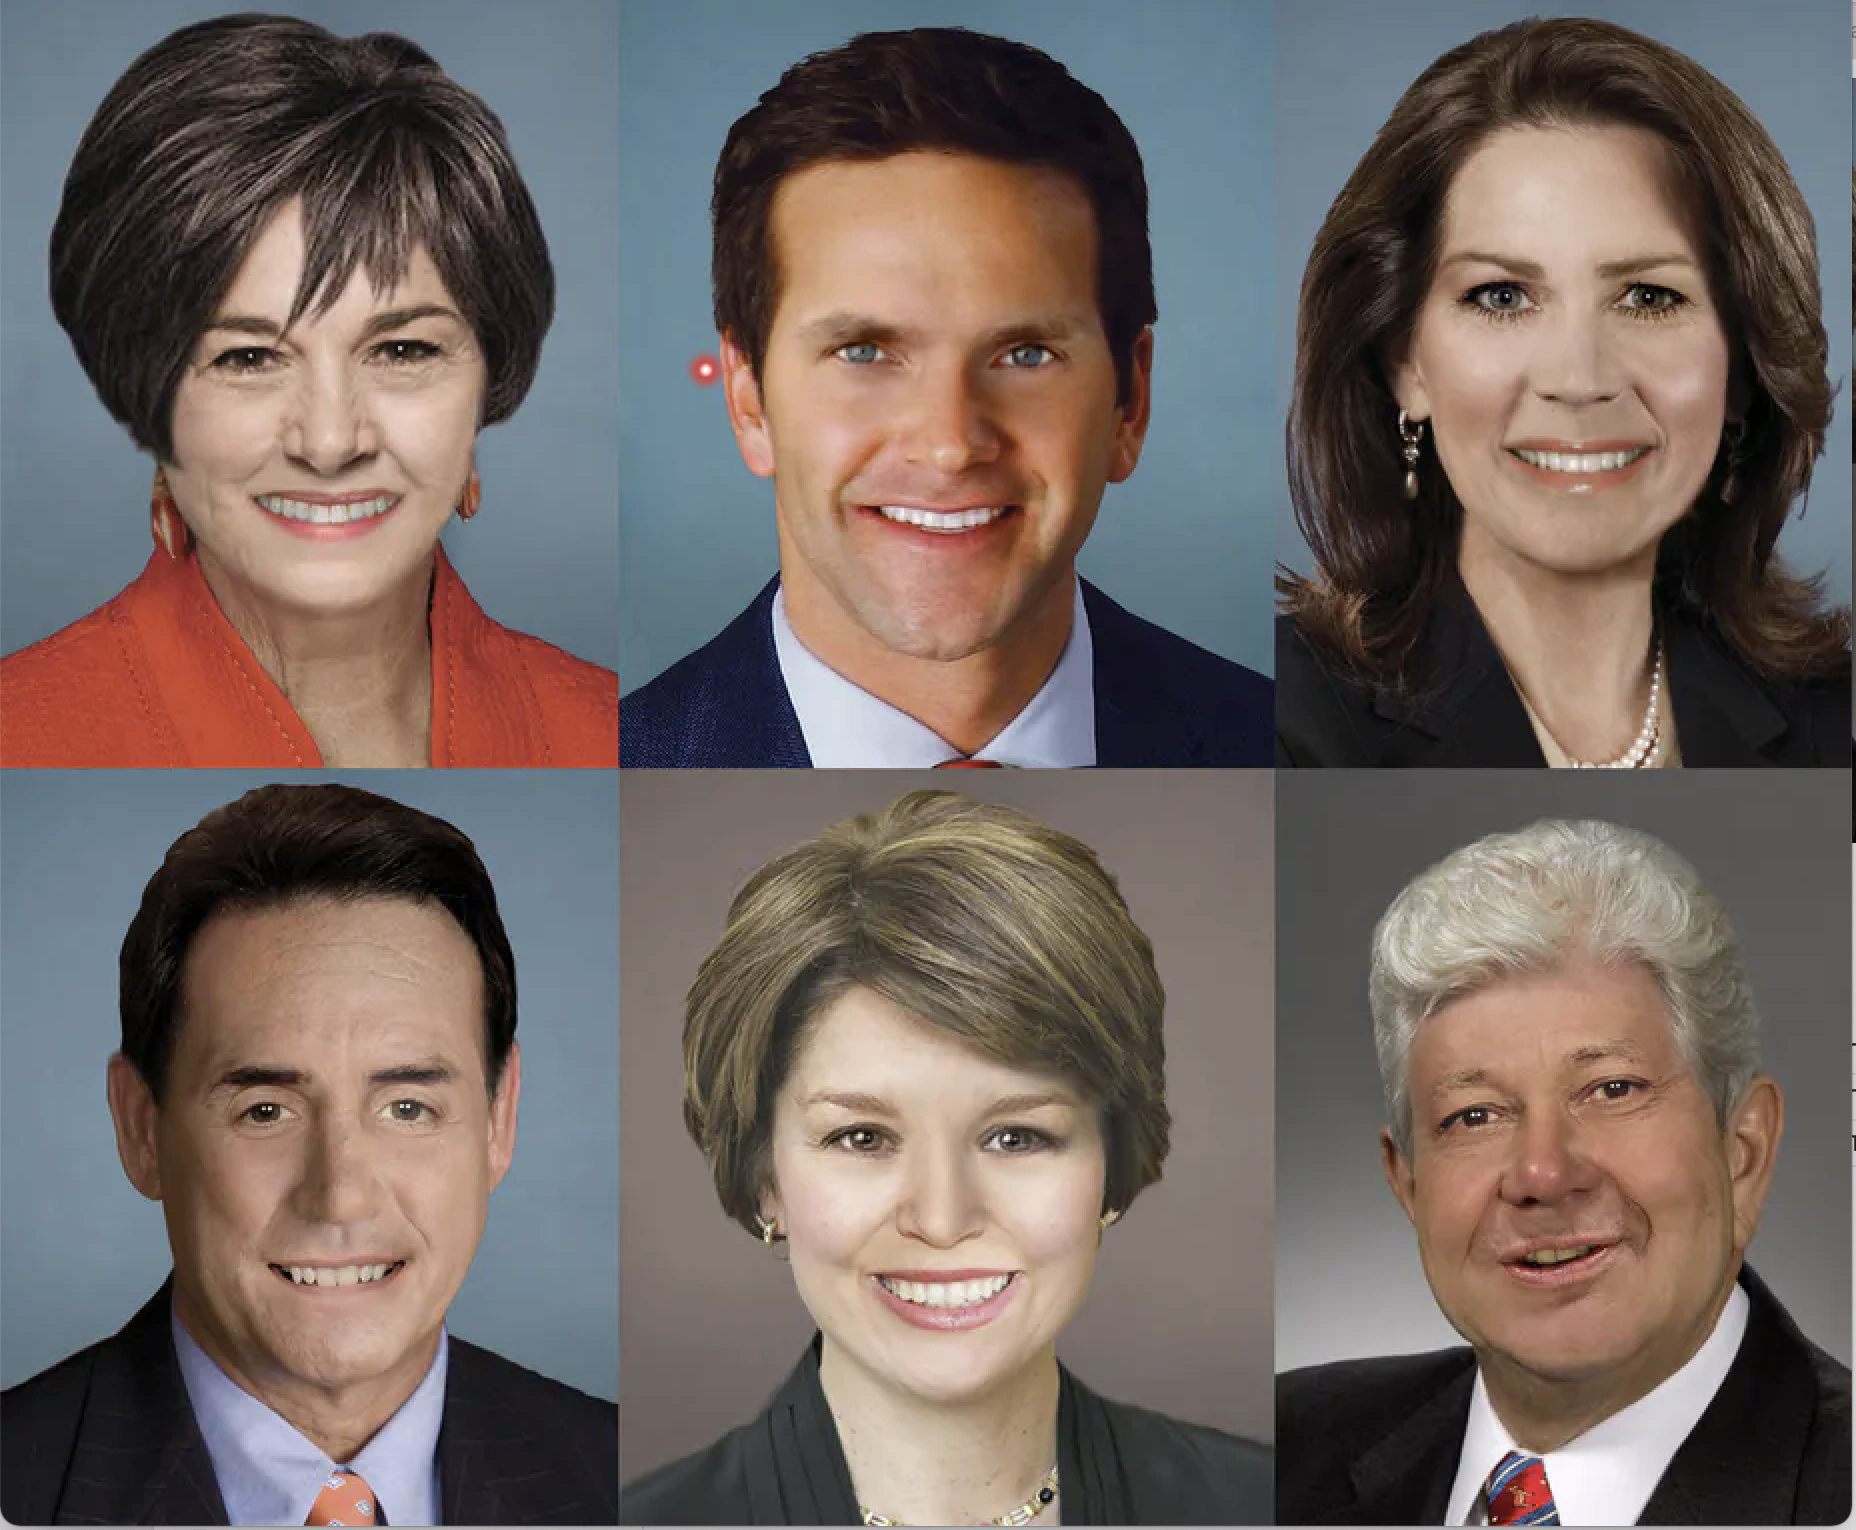
\includegraphics[width=\textwidth]{pic_4.png}
{\tiny ``What Are Good-Looking Candidates?'' (Stockemer and Praino, 2019)}
\end{column}
\end{columns}
\end{frame} 



% 1
\miniframesoff
\begin{frame}[c]{Nixon-Kennedy 1960 Debate}
\begin{columns}
\begin{column}{.45\textwidth}
\begin{itemize}
  \item Nixon's ``five-o'clock'' shadow largely affected voter evaluations.\\{\tiny \color{gray}Mattes et. al (2010).}
  \item[] {\color{white}Nixon didn't look right.}
  \item[] {\color{white}And was all sweaty. {\tiny\color{white} Stockemer and Praino (2019)}.}
  \item[] {\color{white}Radio listeners thought Nixon would win, while TV-watchers though Kennedy would.}
\end{itemize}
\end{column}
\begin{column}{.45\textwidth}
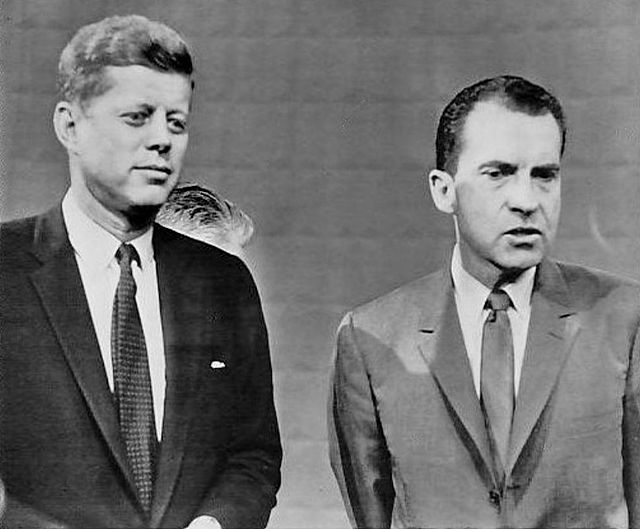
\includegraphics[width=\textwidth]{pic_1.jpg}
\end{column}
\end{columns}
\end{frame} 

% 2
\miniframesoff
\begin{frame}[c]{Nixon-Kennedy 1960 Debate}
\begin{columns}
\begin{column}{.45\textwidth}
\begin{itemize}
  \item Nixon's ``five-o'clock'' shadow largely affected voter evaluations.\\{\tiny\color{gray} Mattes et. al (2010).}
  \item Nixon didn't look right.
  \item[] {\color{white}And was all sweaty. {\tiny\color{white} Stockemer and Praino (2019).}}
  \item[] {\color{white}Radio listeners thought Nixon would win, while TV-watchers though Kennedy would.}
\end{itemize}
\end{column}
\begin{column}{.45\textwidth}
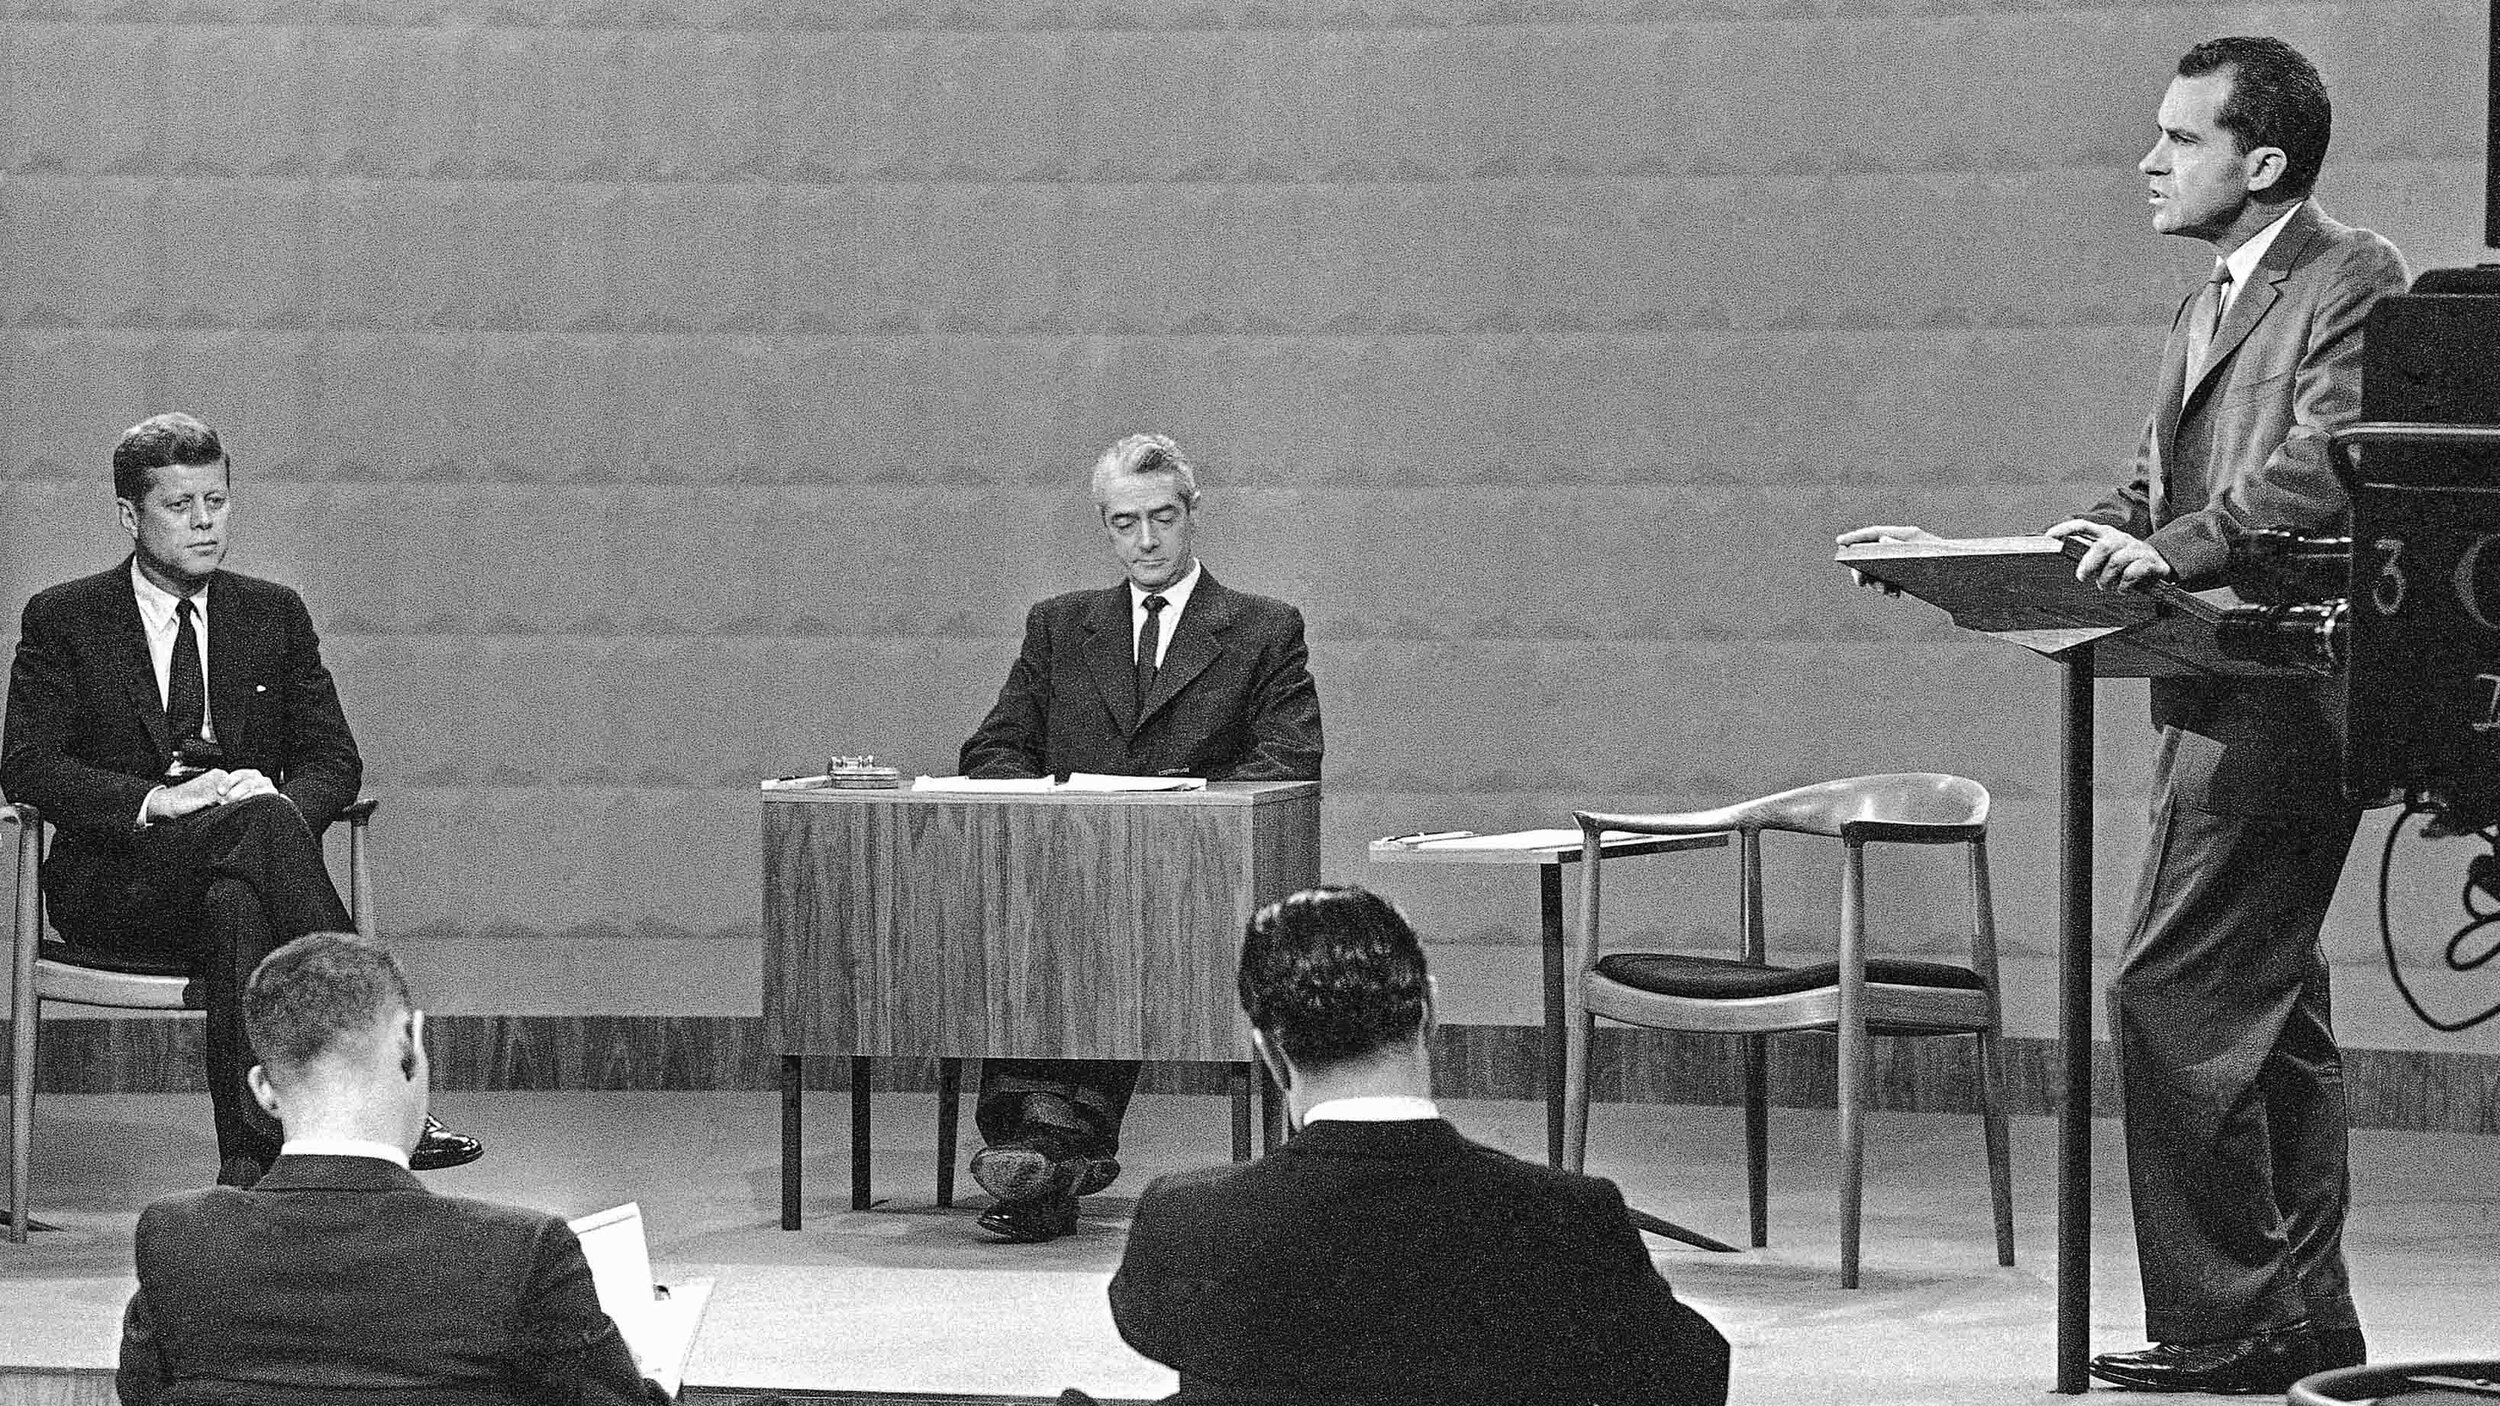
\includegraphics[width=\textwidth]{pic_2.JPG}
\end{column}
\end{columns}
\end{frame} 


% 3
\miniframesoff
\begin{frame}[c]{Nixon-Kennedy 1960 Debate}
\begin{columns}
\begin{column}{.45\textwidth}
\begin{itemize}
  \item Nixon's ``five-o'clock'' shadow largely affected voter evaluations.\\{\tiny \color{gray} Mattes et. al (2010).}
  \item Nixon didn't look right.
  \item And was all sweaty.\\{\tiny\color{gray} Stockemer and Praino (2019).}
  \item[] {\color{white} Radio listeners thought Nixon would win, while TV-watchers though Kennedy would.}
\end{itemize}
\end{column}
\begin{column}{.45\textwidth}
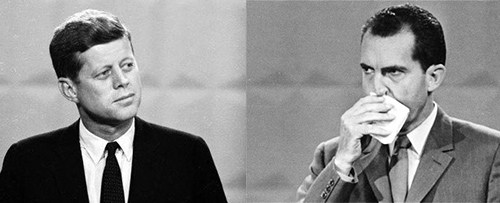
\includegraphics[width=\textwidth]{pic_3.jpg}
\end{column}
\end{columns}
\end{frame} 

% 4
\miniframesoff
\begin{frame}[c]{Nixon-Kennedy 1960 Debate}
\begin{columns}
\begin{column}{.45\textwidth}
\begin{itemize}
  \item Nixon's ``five-o'clock'' shadow largely affected voter evaluations.\\{\tiny \color{gray} Mattes et. al (2010).}
  \item Nixon didn't look right.
  \item And was all sweaty.\\{\tiny\color{gray} Stockemer and Praino (2019).}
  \item Radio listeners thought Nixon would win, while TV-watchers though Kennedy would.
\end{itemize}
\end{column}
\begin{column}{.45\textwidth}
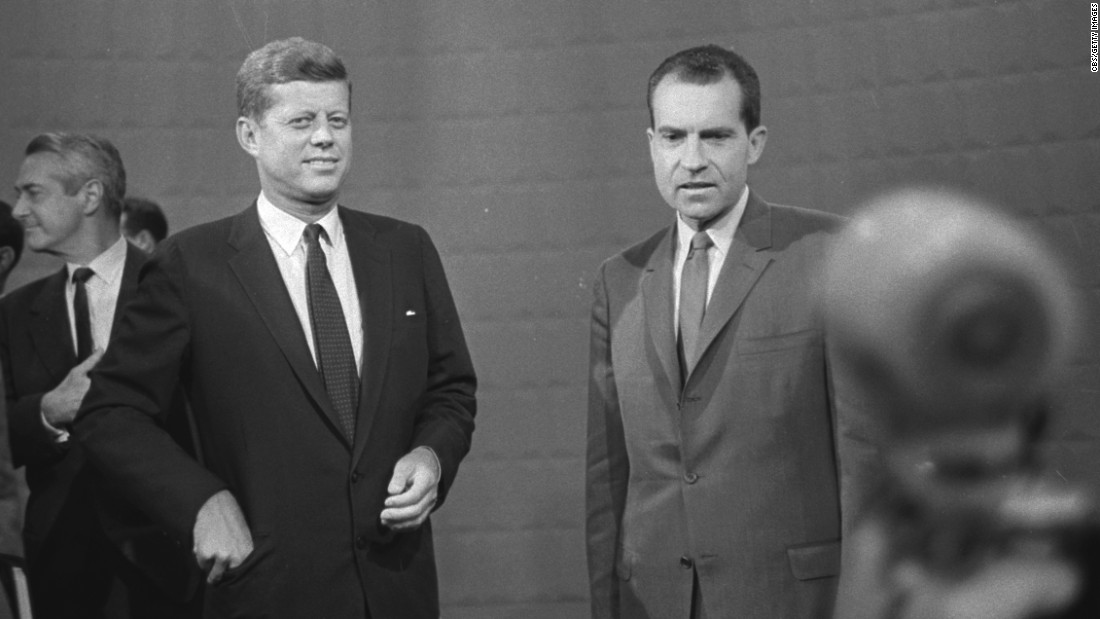
\includegraphics[width=\textwidth]{pic_5.jpg}
\end{column}
\end{columns}
\end{frame} 


\subsection{Gaps}


\miniframeson
\begin{frame}[c]{Gaps in the Current Literature}
\begin{itemize}
  \item While the literature has advanced our knowledge in a number of ways, its focus has been on just attractiveness.
  \item We believe that physical \emph{appearance} goes way beyond than just physical \emph{attractiveness}.
  \item Even while some have studied how ``looking \emph{competent}'' (and not necessarily ``\emph{beautiful}'') helps candidates winning elections, there are a number of unanswered questions.
  \item Importantly, a number of these unexplored questions touch upon issues of social stratification.
  \item For example, \emph{Does it matter for turnout if the candidate looks like a working-class individual as opposed to a white-collar individual?}
\end{itemize}
\end{frame} 


\subsection{Filling in the Gaps}


\miniframeson
\begin{frame}[c]{Our Paper}
\begin{itemize}
  \item Studies the electoral consequences for candidates of looking ``upper-class,'' ``middle-class'' or ``working-class.''
  \item Exploits a novel data set comprised of a representative sample of the Finnish population (N=7,920). In these data, participants rated a subsample of photos of political candidates (N=1,415) according to several physical appearance measurements.
  \item We find that there exists a systematic electoral penalty, particularly for female candidates, that look-like and also hold working-class occupations.
\end{itemize}
\end{frame} 



\section{Theory}

\subsection{Political Psychology and Heuristics}

\miniframeson
\begin{frame}[c]{Political Psychology}
    \begin{itemize}
      \item A candidate's {\bf physical appearance} is ``the most important'' {\color{gray}\tiny (Lau \& Redlawsk 2001)} and the ``most obvious and accessible'' {\color{gray}\tiny (Dion et al. 1972)} \emph{heuristic} available to voters {\color{gray}\tiny (Stockemer \& Praino 2017)}.

      \item {\bf Heuristics} allows reasonable voting decision making with minimal cognitive effort.

      \item Thus, ``voters vote beautiful'' {\color{gray}\tiny(Efrain \& Patterson 1974)} because attractive candidates ``are more likely to be attributed the qualities associated with successful politicians'' {\color{gray}\tiny(Stockemer \& Praino 2019)}.

    \end{itemize}
\end{frame}



\subsection{Expectation States Theory and Inequality}

\miniframeson
\begin{frame}[c]{Expectation States Theory}
    \begin{itemize}
      \item {\bf Expectation States Theory}: physical appearance, gender and occupation ``cue social categories and signify social status'' making them all a ``locus of inequality.''

      - ``sexual attractiveness'' is a gender-specific status symbol: physical attractiveness intersects with gender producing unfavorable outcomes for women.


    \end{itemize}
\end{frame}


\section{Argument}

\subsection{Argument}


\miniframeson
\begin{frame}[c]{Argument}
    \begin{enumerate}

      \item Differences between social groups (gender, occupation, race, etc.) are translated into social inequalities.

      \item For instance, women are more likely to get penalized because of how they look.

      \item In the context of low-information elections, a candidate with a lower status is faced with lower performance expectation, that is, lower turnout. 

      \item Since voters use heuristics, they will elect more systematically high-status male candidates than similar female candidates.

    \end{enumerate}
\end{frame}


\miniframesoff
\begin{frame}[c]%{Argument}
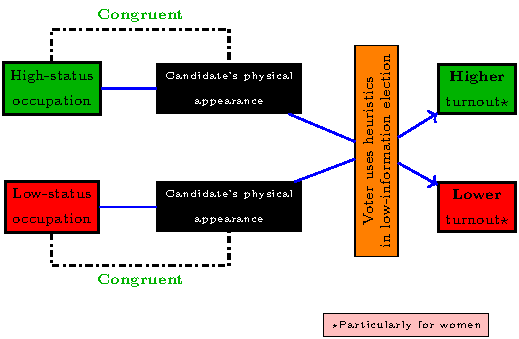
\includegraphics[width=\textwidth]{argument.pdf}
\end{frame}

\section{Empirics}

\subsection{Case}

\miniframeson
\begin{frame}[c]{Finland: A Hard Case}
  \begin{itemize}
    \item We follow a ``{\bf least-likely case design}'' {\color{gray}\tiny(Levy 2008).} Finland has been consistently considered as:
      \begin{itemize}
        \item[-] A democratic {\color{gray}\tiny (Polity-V)}.
        \item[-] An economic egalitarian {\color{gray}\tiny (Waltl 2022)}.
        \item[-] A gender egalitarian.
        \item[-] A social-mobility prone country {\color{gray}\tiny (Erola 2009)}.
        \item[-] Having low-information Municipal Elections {\color{gray}\tiny(Berggren et al. 2010 and 2017)}.
      \end{itemize}
      \item Thus, it should be {\bf hard to find} a correlation between class-congruent use of status symbols and turnout.
    \end{itemize}
\vspace{0.5cm}
{\color{gray}...and yet, we \emph{do}.}
\end{frame}

\miniframeson
\subsection{Data}
\begin{frame}[c]{Several Sources}
  \begin{itemize}
    \item Test.
      \end{itemize}
\end{frame}

\end{document}

